% Figurerne i denne skabelon er fra www.xkcd.com
%
% Brug denne, hvis der printes på begge sider!
\documentclass[a4paper,twoside]{article}
% Brug denne, hvis der kun printes på den ene side!
%\documentclass[a4paper]{article}
\usepackage[utf8]{inputenc}
\usepackage{amsmath}
\usepackage{amsfonts}
\usepackage{amssymb}
\usepackage[danish]{babel} 
\usepackage{graphicx}
\usepackage{subfigure}
\usepackage{float}
% geometry-pakken bruges til f.eks. at ændre margnerne.
% Gør ikke margnerne smallere end dette - Jakob bliver ikke glad!
\usepackage[rmargin=3.2cm,tmargin=3.5cm]{geometry}
% Disse to linjer sikrer, at der bliver mellemrum i stedet for indrykning ved afsnit
\setlength{\parindent}{0pt}
\setlength{\parskip}{1ex plus 0.5ex minus 0.2ex}

% Her begynder selve dokumentet
\begin{document}

% titlepage-miljøet bruges til at sætte en forside op og gør blandt andet at der ikke kommer sidetal
% på og at der automatisk bliver skiftet til en ny side når den er færdig
% At opsætte en forside manuelt kan godt blive lidt kompliceret at se på og man vil derfor ofte
% rykke kode som dette ud i en seperat fil f.eks. forside.tex og inkludere den her med \input{forside}
\begin{titlepage}
\centering
% For forklaring af vspace og stretch, se side 115 i ".. not so short .."
% www.ctan.org/tex-archive/info/lshort/english/lshort.pdf
\vspace*{\stretch{1}}
% rule laver en linje på tværs af siden
\rule{\textwidth}{1mm}\\
\vspace{1cm}
% Her vælger en kæmpe skrifttype og fed skrift
\Huge\bfseries Røntgenståling\\
\vspace{0.7cm}
\rule{\textwidth}{1mm}\\
\vspace{3cm}
\large af\\
Oskar Fugmann (s224073)\\
Mathias Grand (s224070)\\


\vspace{0.7cm}


Gruppenummer: 3
\vspace*{\stretch{2}}
% Nulstiller skriftstørrelse og type (f.eks. fed)
\normalsize
\begin{flushleft}
Rapport i kurset Introduktion til Fysik og nanoteknologi, 10031\\
Danmarks Tekniske Universitet\\
2. Oktober 2022
\end{flushleft}
\end{titlepage}

% Indsætter indholdsfortegelse
\tableofcontents
% Ingen sidetal på siden med indholdsfortegnelsen
\thispagestyle{empty} 
\newpage % Tvunget sideskift for at få indholdsfortegnelsen til at stå på en side for sig selv

\section{Røntgenstråling}
% Tvinger sidetællingen til at starte med 1 på denne side
\setcounter{page}{1} 

% her skal dette med: Teori for røntgenståling og Beskriv dannelsen af røntgenstråling i en anodekilde og herunder hvordan den indsatte krystal tillader måling af intensiteten som funktion af vinkel og dermed energi.
Røntgentstårling er elektromagnetisk stråling med en bølgelængde\
$\lambda \backsim 1\cdot 10^{-10}m\\$
\subsection{Anodekilde}
Røntgen ståling bliver skabt i en anodekilde. En anodekilde består af en katode, som er et stykke af metal hvor i der løber en strøm. Mellem anoden og katoden er der et stor spændingsfald som gør at elektroner fra anoden bliver accelerert op, og skudt in i katoden. Katoden er et stykke metal som bremser elektronen kraftigt op, da den støder ind i katoden, dette skaber en ændring i det elektromagnetiske felt som skaber fotoner, og da energien er tilpashøj bliver røntgenstråling skabt.
\subsection{Absobtion af røntgenstråling}
Når et objekt bestråles med røntgenstråling vil det absobere noget af den stråling. Den mænde som ikke bliver absoberet beskrives ved denne formel og kaldes intensiteten af røntgensttålingen  

\begin{equation}
    I(z)=I_0\cdot e^{-\mu\cdot z}
\end{equation}

hvor $\mu$ er den attenueringskoefficenten og er 
\begin{equation}
    \mu=\frac{\rho\cdot N_a}{M}\cdot\sigma _a 
\end{equation}
hvor $\rho$ er densiteten $N_a$ er Avogadros tal og $M$ er Molarmassen og $\sigma _a$ beskriver sandsynligheden for at et atom absobere en røntgensfoton og $\sigma _a =(Z^4,E_\lambda^{-3})$

\subsubsection{Absobtionskanter}
Når et atom bestråles med røntgenstråling vil intensiteten som funktion af energien. Der sker dog det, at ved bestemte energier vil røntgenstrålingen kunne slå en elektron ud af en skal. Dette gør at sandsynligeheden for vekselvirkning mellem atom og røntgenstråling stiger, altså stiger absobtionen. 

\subsection{Bremsestråling}
Når en elektron rammer adonematrialet i et anoderør, vil der blive skabt en foton. Dette klades også bremsestråling, som er når en elektron oplever en acceleration og udsender en foton. Energien af fotoen er bestemt med denne som
\begin{equation}
    E_{foton}=E_2-E_1=h\cdot v
    \end{equation}
hvor $h$ er Placks konstant og $v$ er frekvensen. Sandsyndligheden for en given energiædning, bliver lavere ved større endergiendringer.

\subsection{Karaterisktisk stråling}
Hvis en elektron har en energi større end bindingsenergien for en elektron i anodematrialet, kan elektronen i anodematrialet, blive løsrevet. Dette skaber et hul, som vil udfyldt af en elektron fra en ydre skal, og vil udsende en foton med en bestem energi, som er specifik for anodematrialet og den skal, som elektronen forsvandt fra. Skallerne navngives K, L, M, N (inde fra og ude), hvor det kræver mest energi at løsriven en elektron i en K skal og mindst i en N skal grundet bindingsenergien

\subsection{Røngten spektrum}
Ved udnyttelse af bremsestråling og karaterisktisk stråling kan man bestemme matrialer udfra røngtenstråling. Med linært aftagnede bramsetråling, den karakteristike stråling. Ved leve værdier for energien af røntgenstråling vil lufte absobere store dele af streålingen og den vil derfro ikke følge den linære bremsetråling.

\subsection{Interfrens}
Hvis en krystal bestråles med røntgenstråling vil krystalgitteret fungere som et gitter laver interfrens. Den afbøjningsvinkel hvor der konstruktive interfrens er udtrykt ved bragslov $2\cdot d \cdot sin(\Theta)=n\cdot \lambda$. Energien af en foton er beskrivet med denne formel: $E=\frac{h\cdot}{\lamda}$. Dermed er erngien for udtrykt ved afbøjningsvinklen 
\begin{equation}
    E=\frac{n\cdot h\cdot c}{2\cdot d\cdot sin(\Theta)}
\end{equation}



\begin{figure}
\begin{centering}
\includegraphics[width=0.9\columnwidth]{}
\par\end{centering}
\caption{\label{cap:nerd_sniping}Et eksempel på en figur. Husk at figuren skal indeholde en selvforklarende figurtekst.}
\end{figure}

\section{Opstiling af forsøgene}
%Oskar og Mathias
%Beskriv den eksperimentelle opstilling (husk en skitse) og beskriv de opnåede resultater fra deløvelse 1a grafisk og beskriv den eksperimentelle opstilling (husk en skitse)



\section{2-D billede analyse}
%Mathias

\section{Databehandling af 3-D billeder} 
%Oskar

\chapter{Eksperimentel øvelse 2}


\section{Intensiteten som funktion af røngtenenergi for kun krystal}
%mathias
%Vis en graf over I(E), dvs. intensiteten af den spredte stråling I som funktion af røntgen- energien E for eksperimentet uden filter 
% Kommenter på de karakteristiske elementer af I(E)

\begin{figure}[H]
\begin{centering}
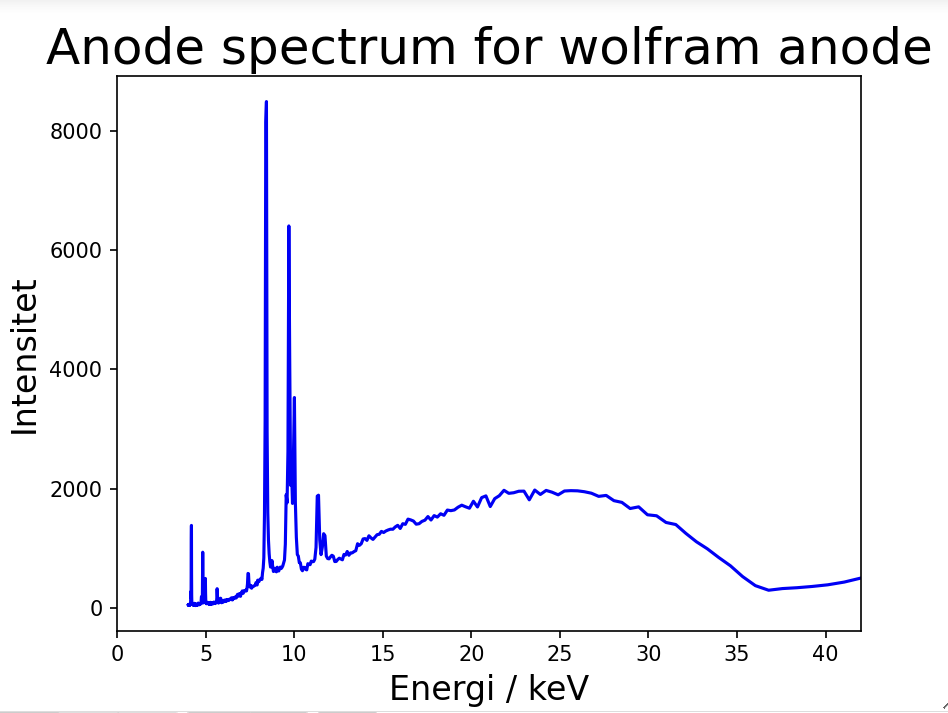
\includegraphics[height=5cm]{Wolfram krystal.png}
\includegraphics[height=5cm]{zoomed in.png}
\hspace{1cm}
\par\end{centering}
\caption{\label{cap:2ien} Anode spectrum for wolfram krystal uden filter }
\end{figure}
Ved anvendelse af vores pythonprogram, hvor grafen er konstrueret kan vi bestemme ved hvilke værdier der er karakteristisk stråling, og eftertjekke det med de udleveret værdier. 
\\ På det udleverede dokument over absorbtions og emmissions energier for wolfram. Her ligger K springende ved for høje energi niveauer. Disse vises ikke da vores røngten stråle "kun" var på 35keV mens K springende ligger omkring 60keV. De andre burde være mulige. I tabellen under er de målte værdier sat op overfor de angivet for kartakteristk stråling for wolfram. Enheden i tabellen er eV. 
\begin{center}
\begin{tabular}{||c c c ||} 
 \hline
 Type for tabel værdien & Tabel værdi & Målt værdi \\ [0.5ex] 
 \hline\hline
 $L_{\gamma1}$ & 11286 & 11340  \\ 
 \hline
  $L_{\beta2}$ & 9956 & 10014 \\ 
 \hline
$L_{\beta3}$ & 9819  & 9850  \\
 \hline
 $L_{\beta1}$ & 9673 & 9692 \\ [1ex] 
 \hline
 $L_{\beta4}$ & 9525 & 9548 \\
 \hline
 $L_{\alpha1}$ & 8398 & 8400 \\ [1ex] 
  \hline
 & & 7380 \\ [1ex] 
  \hline
 & & 4960 \\ [1ex]  
 \hline
  & & 4830 \\ [1ex] 
 \hline
  & & 4190\\ [ex] 
 \hline
\end{tabular}
\end{center}
På tabellen kan det ses, at nogle af værdierne ligger meget tæt på hinanden. Det var ikke muligt, at se alle spectral linjerne indtil man zoomede ind i intervallet 8-10, da der her ligger linjerne rigtigt tætte. Det ser ud som om vi har fundet alle de karakteristiske linjer der er angivet på det udleveret ark. Derudover har vi fundet nogle spikes ved energier som ikke er på det udlevereret ark. (Spørge til kursus onsdag)\\
\\Grafen burde gå i 0 ved 35keV, da det er den energi elektronerne accelereres til. Det skyldes at vores sensor ikke kan måle energierne af de fotoner der rammer men blot tæller hvor mange der rammer, men i stedet er udregnet ved diffraktion gennem krystalstruktur ved måling af diffraktionsvinklen. De høje energier er fundet ved små vinkler og derfor kan røngten strålingen have ramt sensoren uden at lave differaktion med crystallen.
\section{Vinkel for metaler og intensitet}
\begin{figure}[H]
\begin{centering}
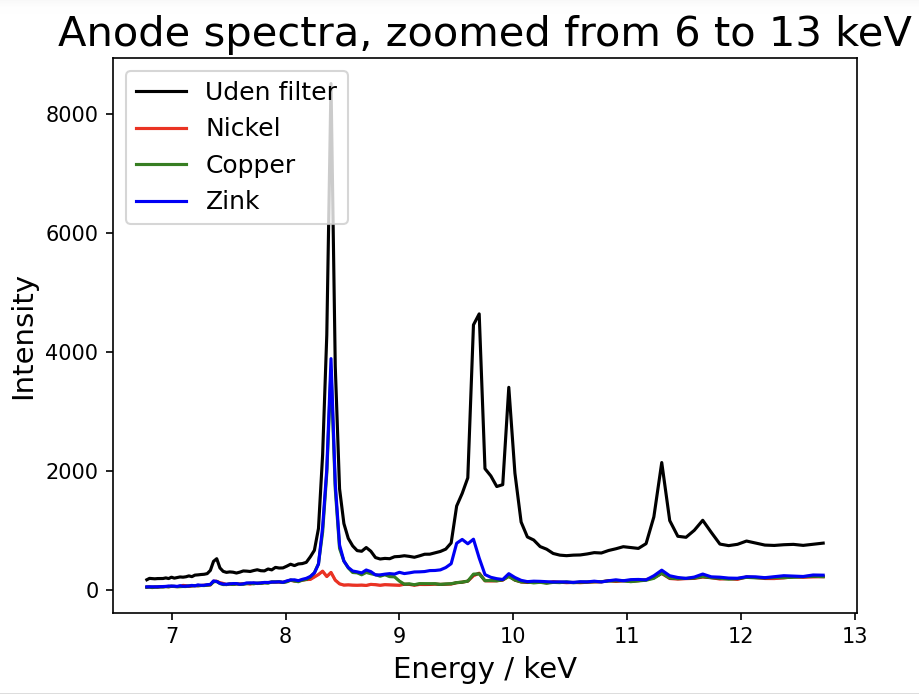
\includegraphics[height=6cm]{Anode spectra.png}
\hspace{1cm}
\par\end{centering}
\caption{\label{cap:2ien} Anode spectrum for wolfram med forskellige filtre }
\end{figure}
Filteret gør at der generelt kommer mindre stråling igennem, da  fotonerne skal passere mere stof. Der må være en spike, hvis der ikke sker karakteristik stråling i filteret, da ellers vil meget af denne energi istedet løsrive elektroner i filteret fremfor at ramme detektoren. Vi kan se ved den første store spike på grafen uden filter er Nickel den eneste der ikke spiker. Det skyldes at der også sker karakteristisk stråling i Nickel ved denne energi. Nemlig 8.3 keV for $K_{edge}$. De andre har stadig en spike, da deres karakteristiske værdier ligger lidt over. Nickel fortsætter derefter med konstant at ligge cirka samme sted. Copper kommer ned og møder nickel ved værdien 8.9 keV som også er her den har $K_{edge}$. Til sidst kan det ses at Zinks absorbtion stiger ved 9.6 keV som også er her $K_{edge}$ ligger for zinc. Det er det samme som kan ses i figuren nedenfor. 


\begin{figure}[H]
\begin{centering}
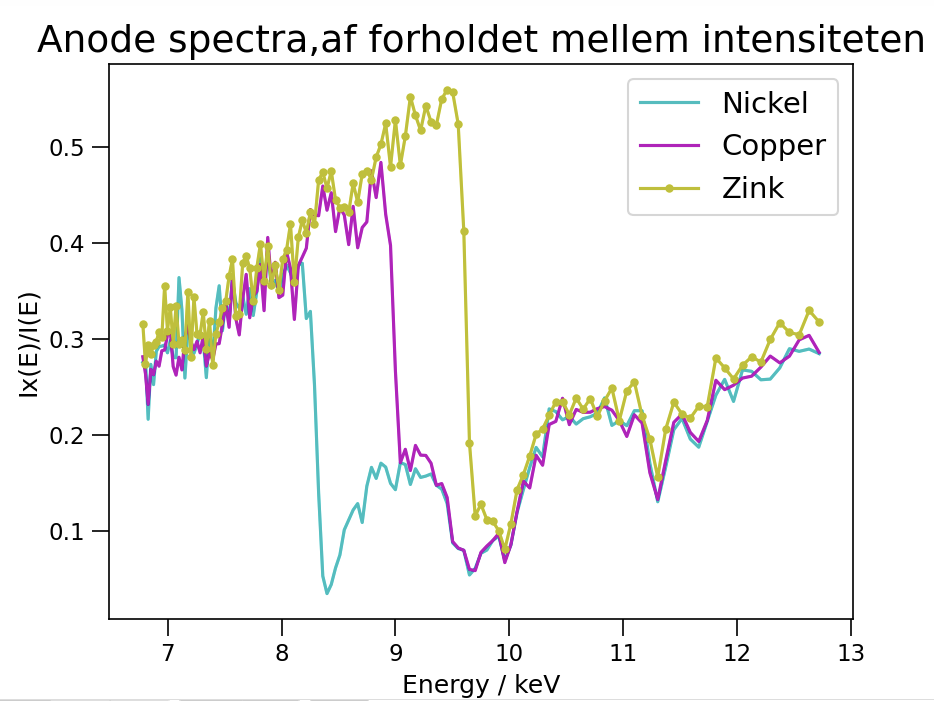
\includegraphics[height=6cm]{Anode spectra forhold mellem intensiteterne.png}
\hspace{1cm}
\par\end{centering}
\caption{\label{cap:2ien} Anode spectrum af forholdet mellem I og $I_0$ }
\end{figure}
Nickel, Copper og Zink ligger lige efter hinanden i det periodiske system, derfor er deres attenueringskonstant meget ens og det er deres densitet også. Derfor følger de hinanden meget godt alle de steder der ikke skyldes karakteristisk stråling. 
\\ Hvis vi kigger de steder der skere drastiske fald, skyldes det karakteristik stråling. Kigger vi ved energierne på energierne stemmer det over med $K_{edge}$. For Nickel er den 8333 eV, Copper er 8979 eV og Zink 9659 eV. (Spørg om det er Kalpha eller edge) \\
Der sker et fald her, fordi fotonerne har netop den energi der kræves for at løsrive en elektron, og derfor absorberes stråligen og derfor falder I mens $I_0$ er uændret. 
\\
Det kan også ses, at graferne er stigende før og efter deres store fald. Hvilket skyldes at en stigning i foton energien medførerer en formindskning i attenueringskoefficienten og dermed stiger forholdet mellem start og slut intensitet. 

%mathias
% Vis I(E) for alle de fire udførte scans (Iuden (E), INi (E), ICu (E), IZn (E)), kommenter på interessante forskelle og ligheder målingerne imellem 
% Beregn og plot IX (E)/ I(E), hvor X=[Ni, Cu, Zn], og kommenter på resultatet.t

\section{Opgaver}
% de 8 opgaver som skal løses
\subsection{\bold{Opgave 1}}
\subsubsection*{Hvad er energien af en elektron, efter at den krydset et anode/katodegab med et spændingsfald på 20 kV? -Antag, at elektronen starter fra hvile, og angiv resultatet i
både elektronvolt og joule?}
Definationen af en elektronvolt er den energi en elektron opnår, når den passere et spændingsfald på $1V$. Derfor må elektronen opnå en energi på $20keV$. For at omdanne det til joule skal vi multiplicerer med $1,602\cdot10^{-19} \frac{J}{eV}$, som er omskrivningsfaktoren
\begin{equation*}
20\cdot10^3 eV \cdot1,602\cdot10^{-19} \frac{J}{eV}=3.2\cdot10^{-15} J
\end {equation*}

\subsection{\bold{Opgave 2}}
\subsubsection*{Hvad er hastigheden af en elektron med den ovenfor beregnede energi?}
Den ovenfor beregnede energi er elektronens kinetiske energi, og vi kan derfor finde dens fart som $v=\sqrt{\frac{2E}{m}}$.
Det vides at elektronens masse er $9,11\cdot10^{-31} kg$

\begin {equation*}
v=\sqrt{\frac{2\cdot3.2\cdot10^{-15}J}{9.11\cdot10^{-31}kg}}=8.4\cdot10^7 \frac{m}{s}
\end{equation*}
\subsection{\bold{Opgave 3}}
Vi skal finde den samlet effekt som røngtenkilden udsender og så finde 1 promile af den 
\begin{equation*}
35kV\cdot1,0mA=35W
\end{equation*}
\begin{equation*}
    35W\cdot0,001=0,035W
\end{equation*}
Vi ved at den energi der kræves for at lave $K_{\alpha1}$ er $17480eV$ for molybdæn, det skal vi lave om til Joule og det skal dividerer med promilen af effekten for at finde antalet af udsendte funktioner pr. sekund
\begin{equation}
    17480eV=2.80\cdot10^{-15}J
\end{equation}
\begin{equation*}
     \frac{0,035W}{2.80\cdot10^{-15}J}=1.25\cdot10^{13}\frac{fotoner}{s} 
\end{equation*}
Der udsendes $1.25\cdot10^{13}$ $k_{\alpha1}$ fotoner pr. sekund
\subsection{\bold{Opgave 4}}
Først skal jeg finde attenueringskoefficienten for vand, calcium og bly. På (indsæt reference) kan jeg finde den ved forskellige foton energier. Jeg vælger fotonenergien 15keV, da det ligger tættest $k_{\alpha}$ fra sidste opgave. Samt multiplicerer med densiteten, da den fundne attenueringskonstant afhænger af densiteten.
Vand: $1.673 \frac{cm^2}{g}$
\begin{equation*}
    \mu_{vand}=1.673 \frac{cm^2}{g}\cdot0.997 \frac{g}{cm^3}=1.6680 cm^{-1}
\end{equation*}
De andre er fundet lige ledes og kan findes under appendix
For at plotte det skal jeg finde $I_0$
Vi har antallet af fotoner fra sidste opgave men kun 1\% fotonerne rammer prøven. 
\begin{equation*}
   I_0= 1.25\cdot10^{13}\cdot0.01=1.25\cdot10^{11} 
 
\end{equation*}
Vi har valgt at samle graferne så de kan sammenlignes. Derfor skal vi nu gøre det samme for et nyt anode materiale nemlig Wolfram. 
Udregningerne kan ses i samme appendix

  Graferne kan nu blottes med formlen
  \begin{equation}
      I=I_0\cdot e^{-\mu*x}
  \end{equation}

\begin{figure}[H]
\begin{centering}
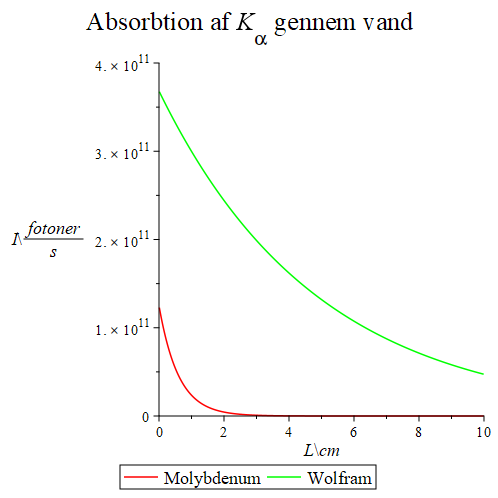
\includegraphics[height=4.15cm]{Absorbtion gennem vand.png}
\hspace{0.5cm}
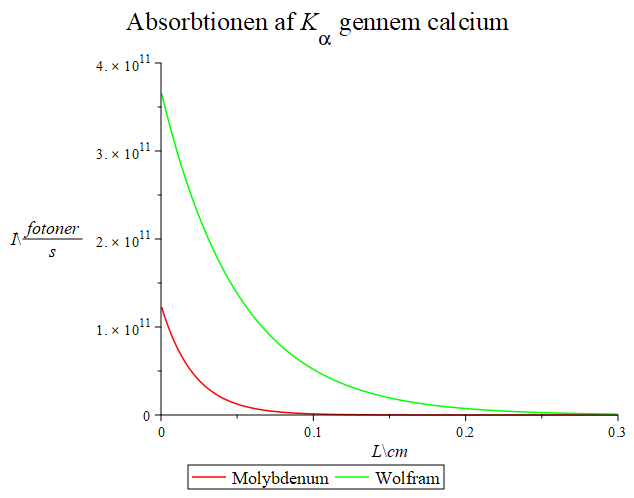
\includegraphics[height=4.15cm]{Absorbtion gennem calcium.png}
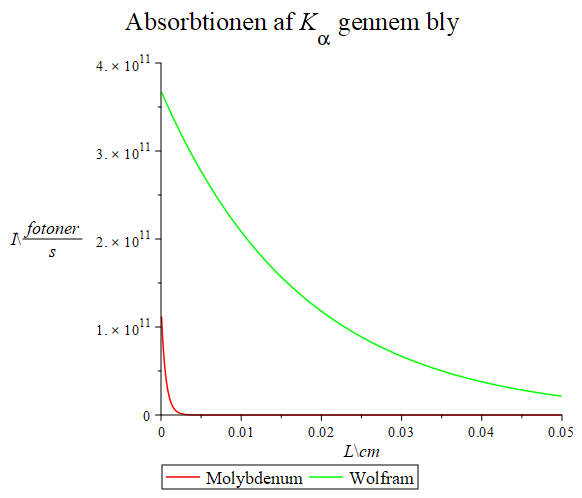
\includegraphics[height=4.15cm]{Absorbtion gennem bly.png}
\par\end{centering}
\caption{\label{cap:2ien} Grafer over absorbtion af $K_{\alpha1}$ }
\end{figure}
Problemet ved at andvende en molybdæn er at hvis man skal bruge det til at tage røngten fotografier af mennesker med, kan røngtenstrålerne ikke passerer få cm vand eller calcium, hvilket vil betyde at hvis man skal teste for fx en brækket arm vil kontrasten mellem knogle og væske i kroppen værre meget lille, da næsten alt røngtenstrålingen absorberes inden det når igennem armen. Mens wolfram godt kan passerer vand rimeligt godt, men ikke calcium og dermed vil der opstå en større konstrast mellem de to på et røngten fotografi. Hverken af dem kan dog passerer bly, men det har ikke de store problemer inden for medicinsk billededannelse, da kroppen ikke består af store mængder af bly. 
\subsection{\bold{Opgave 5}}
Vi løser opgaven med denne formel $\frac{I(z)}{I_0}=e^{-\mu z}$. vi finder $\mu\over\rho$ i Nist til $2,032\cdot 10^{-1} \frac{g}{cm^2}$ og densiteten af Polymethyl Methacrylate til at være $1,18\frac{cm^3}{g}$\\
$\mu$ findes
\begin{equation*}
    \mu=2,032\cdot10^{-1}\frac{g}{cm^2}\cdot1,18\frac{cm^3}{g}=0,24cm^{-1}
\end{equation*}
$I(z)\over Z_0$ findes
\begin{equation*}
    \frac{I(z)}{I_0}=e^{-0,24cm^{-1}\cdot 1cm}=0,79
\end{equation*}
 
    Dermed kommer $79\%$ igennem prøven\\
Hvis $1\%$ er bly kan vi beskrive det som $\frac{I(z_1+z_2)}{I_0}=e^{-\mu_1\cdot z_1-\mu_2 z_2}$ hvor $z_1=0,99cm$ og $z_2=0,01cm$. Vi finder $\mu$ for bly, vi finder i nist at $3,032\cdot10^1$ og densiteten af bly findes til $10,66\frac{g}{cm^3}$
\begin{equation*}
    \mu=2,032\cdot10^{1}\frac{g}{cm^2}\cdot10,66\frac{cm^3}{g}=21216,6cm^{-1}
\end{equation*}
$I(z)\over Z_0$ findes
\begin{equation*}
    \frac{I(z)}{I_0}=e^{-0,24cm^{-1}\cdot 0,99cm - 21216,6cm^{-1}\cdot 0,01cm}=0,09
\end{equation*}
Dermed kommer $9\%$ af strålingen igennem




\subsection{\bold{Opgave 6}}
\subsubsection*{Den direkte røntgenstråle fra en moderne synkrotronkilde kan have op til $10^{17} \frac{fotoner}{sekund}$ med en foton-energi på $30keV$. Hvad er effekten $P$, udtrykt i watt, af en sådan stråle?}
For at finde effekten skal vi finde strålens samlet energi pr. s. Derfor skal vi multiplicerer antallet af fotoner pr. sekund med foton-energien 
\begin{equation*}
P=10^{17}*\frac{fotoner}{sekund}\cdot30\cdot10^{3}eV\cdot1.602\cdot10^{-19} \frac{J}{eV}=480.6W
\end{equation*}
    
\subsection{\bold{Opgave 7}}
Først skal vi finde effekten pr. areal af strålen. 
\begin{equation*}
    \frac{480.6W}{2\cdot10^{-6}m^2}=2.40\cdot10^{8}

\end{equation*}
Jeg antager at hele kogepladen dækker $0.25 m^2$
\begin{equation*}
    \frac{2.40\cdot10^{8}}{\frac{2\cdot10^3W}{0.25m^2}}=30038
\end{equation*}
Effekten pr. areal er cirka 30000 gange større for røngtenstrålen end for en kogepålade med en effekt på 2kWh

\subsection{\bold{Opgave 8}}
For at løse opgaven skal jeg først bestemme Attenueringskoefficienten som jeg finder ved (indsæt reference)
\subsubsection*{}For 30keV

\begin{equation*}
    30.32\frac{cm^2}{g}\cdot19.3\frac{g}{cm^3}=585.18cm^{-1}
\end{equation*}
For 100 keV
\begin{equation*}
    5.549\frac{cm^2}{g}\cdot19.3\frac{g}{cm^3}=107.10cm^{-1}
\end{equation*}
Nu indsætter vi værdierne i absorbtionsloven og finder tykkelsen der netop giver I=1. Tykkelsen der netop er større end den værdi må dermed "stoppe" strålen. 
\begin{equation*}
  1=10^{17}\cdot e^{585.18cm^{-1}\cdot x}
\end{equation*}
\begin{equation*}
    x=0.067
\end{equation*}
For 100 keV
\begin{equation*}
     1=10^{17}\cdot e^{107.10cm^{-1}\cdot x}
\end{equation*}
\begin{equation*}
    x=0.366
\end{equation*}
\newpage
\section{}
%\bibliographystyle{plain} - hvis I bruger BibTeX lsningen
%\bibliography{skabelon_bib}

\begin{thebibliography}{} % det simple alternativ til BibTeX
\bibitem{collins2000}
Phillip G. Collins and Phaedon Avouris, Scientific American, \textbf{283}, 62 (2000)
\end{thebibliography}

\newpage 

\appendix
\section{Appendix-overskrift}
Denne tekst står i det første appendix

https://www.nist.gov/pml/x-ray-mass-attenuation-coefficients


\section{Flere udregninger i opgaver 4}
\begin{figure}[H]
\begin{centering}
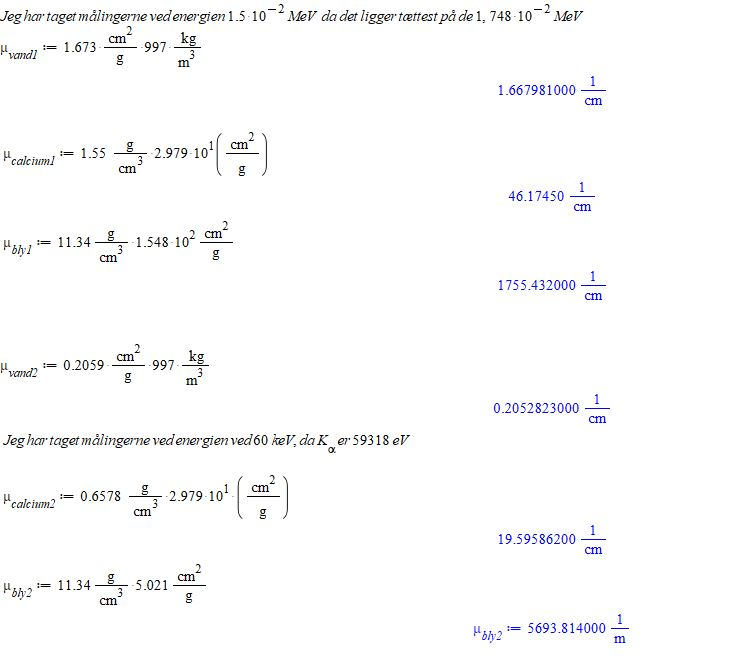
\includegraphics[height=14cm]{Opgave 4.jpg}
\hspace{1cm}
\par\end{centering}
\caption{\label{cap:2ien} Anode spectrum af forholdet mellem I og $I_0$ }
\end{figure}




\section{Fordeling af arbejde}
% her skal vi have documentet med arbejdsfordelingen så forlæsere kan se hvad ved har lavet
\end{document}
